% Options for packages loaded elsewhere
\PassOptionsToPackage{unicode}{hyperref}
\PassOptionsToPackage{hyphens}{url}
%
\documentclass[
  xelatex,ja=standard]{bxjsarticle}
\usepackage{lmodern}
\usepackage{amssymb,amsmath}
\usepackage{ifxetex,ifluatex}
\ifnum 0\ifxetex 1\fi\ifluatex 1\fi=0 % if pdftex
  \usepackage[T1]{fontenc}
  \usepackage[utf8]{inputenc}
  \usepackage{textcomp} % provide euro and other symbols
\else % if luatex or xetex
  \usepackage{unicode-math}
  \defaultfontfeatures{Scale=MatchLowercase}
  \defaultfontfeatures[\rmfamily]{Ligatures=TeX,Scale=1}
\fi
% Use upquote if available, for straight quotes in verbatim environments
\IfFileExists{upquote.sty}{\usepackage{upquote}}{}
\IfFileExists{microtype.sty}{% use microtype if available
  \usepackage[]{microtype}
  \UseMicrotypeSet[protrusion]{basicmath} % disable protrusion for tt fonts
}{}
\makeatletter
\@ifundefined{KOMAClassName}{% if non-KOMA class
  \IfFileExists{parskip.sty}{%
    \usepackage{parskip}
  }{% else
    \setlength{\parindent}{0pt}
    \setlength{\parskip}{6pt plus 2pt minus 1pt}}
}{% if KOMA class
  \KOMAoptions{parskip=half}}
\makeatother
\usepackage{xcolor}
\IfFileExists{xurl.sty}{\usepackage{xurl}}{} % add URL line breaks if available
\IfFileExists{bookmark.sty}{\usepackage{bookmark}}{\usepackage{hyperref}}
\hypersetup{
  pdftitle={Making maps and analysing spatial data: An introduction to using R for archaeologists/考古学者のためのRによる地図作成と空間データ分析},
  pdfauthor={Liying Wang; Atsushi Noguchi (translator)},
  hidelinks,
  pdfcreator={LaTeX via pandoc}}
\urlstyle{same} % disable monospaced font for URLs
\usepackage[no]{geometry}
\usepackage{color}
\usepackage{fancyvrb}
\newcommand{\VerbBar}{|}
\newcommand{\VERB}{\Verb[commandchars=\\\{\}]}
\DefineVerbatimEnvironment{Highlighting}{Verbatim}{commandchars=\\\{\}}
% Add ',fontsize=\small' for more characters per line
\usepackage{framed}
\definecolor{shadecolor}{RGB}{248,248,248}
\newenvironment{Shaded}{\begin{snugshade}}{\end{snugshade}}
\newcommand{\AlertTok}[1]{\textcolor[rgb]{0.94,0.16,0.16}{#1}}
\newcommand{\AnnotationTok}[1]{\textcolor[rgb]{0.56,0.35,0.01}{\textbf{\textit{#1}}}}
\newcommand{\AttributeTok}[1]{\textcolor[rgb]{0.77,0.63,0.00}{#1}}
\newcommand{\BaseNTok}[1]{\textcolor[rgb]{0.00,0.00,0.81}{#1}}
\newcommand{\BuiltInTok}[1]{#1}
\newcommand{\CharTok}[1]{\textcolor[rgb]{0.31,0.60,0.02}{#1}}
\newcommand{\CommentTok}[1]{\textcolor[rgb]{0.56,0.35,0.01}{\textit{#1}}}
\newcommand{\CommentVarTok}[1]{\textcolor[rgb]{0.56,0.35,0.01}{\textbf{\textit{#1}}}}
\newcommand{\ConstantTok}[1]{\textcolor[rgb]{0.00,0.00,0.00}{#1}}
\newcommand{\ControlFlowTok}[1]{\textcolor[rgb]{0.13,0.29,0.53}{\textbf{#1}}}
\newcommand{\DataTypeTok}[1]{\textcolor[rgb]{0.13,0.29,0.53}{#1}}
\newcommand{\DecValTok}[1]{\textcolor[rgb]{0.00,0.00,0.81}{#1}}
\newcommand{\DocumentationTok}[1]{\textcolor[rgb]{0.56,0.35,0.01}{\textbf{\textit{#1}}}}
\newcommand{\ErrorTok}[1]{\textcolor[rgb]{0.64,0.00,0.00}{\textbf{#1}}}
\newcommand{\ExtensionTok}[1]{#1}
\newcommand{\FloatTok}[1]{\textcolor[rgb]{0.00,0.00,0.81}{#1}}
\newcommand{\FunctionTok}[1]{\textcolor[rgb]{0.00,0.00,0.00}{#1}}
\newcommand{\ImportTok}[1]{#1}
\newcommand{\InformationTok}[1]{\textcolor[rgb]{0.56,0.35,0.01}{\textbf{\textit{#1}}}}
\newcommand{\KeywordTok}[1]{\textcolor[rgb]{0.13,0.29,0.53}{\textbf{#1}}}
\newcommand{\NormalTok}[1]{#1}
\newcommand{\OperatorTok}[1]{\textcolor[rgb]{0.81,0.36,0.00}{\textbf{#1}}}
\newcommand{\OtherTok}[1]{\textcolor[rgb]{0.56,0.35,0.01}{#1}}
\newcommand{\PreprocessorTok}[1]{\textcolor[rgb]{0.56,0.35,0.01}{\textit{#1}}}
\newcommand{\RegionMarkerTok}[1]{#1}
\newcommand{\SpecialCharTok}[1]{\textcolor[rgb]{0.00,0.00,0.00}{#1}}
\newcommand{\SpecialStringTok}[1]{\textcolor[rgb]{0.31,0.60,0.02}{#1}}
\newcommand{\StringTok}[1]{\textcolor[rgb]{0.31,0.60,0.02}{#1}}
\newcommand{\VariableTok}[1]{\textcolor[rgb]{0.00,0.00,0.00}{#1}}
\newcommand{\VerbatimStringTok}[1]{\textcolor[rgb]{0.31,0.60,0.02}{#1}}
\newcommand{\WarningTok}[1]{\textcolor[rgb]{0.56,0.35,0.01}{\textbf{\textit{#1}}}}
\usepackage{graphicx,grffile}
\makeatletter
\def\maxwidth{\ifdim\Gin@nat@width>\linewidth\linewidth\else\Gin@nat@width\fi}
\def\maxheight{\ifdim\Gin@nat@height>\textheight\textheight\else\Gin@nat@height\fi}
\makeatother
% Scale images if necessary, so that they will not overflow the page
% margins by default, and it is still possible to overwrite the defaults
% using explicit options in \includegraphics[width, height, ...]{}
\setkeys{Gin}{width=\maxwidth,height=\maxheight,keepaspectratio}
% Set default figure placement to htbp
\makeatletter
\def\fps@figure{htbp}
\makeatother
\setlength{\emergencystretch}{3em} % prevent overfull lines
\providecommand{\tightlist}{%
  \setlength{\itemsep}{0pt}\setlength{\parskip}{0pt}}
\setcounter{secnumdepth}{-\maxdimen} % remove section numbering

\title{Making maps and analysing spatial data: An introduction to using R for
archaeologists/考古学者のためのRによる地図作成と空間データ分析}
\author{Liying Wang \and Atsushi Noguchi (translator)}
\date{6/14/2020}

\begin{document}
\maketitle

\hypertarget{introductionux306fux3058ux3081ux306b}{%
\section{Introduction/はじめに}\label{introductionux306fux3058ux3081ux306b}}

In this workshop, you will learn how to use R to manipulate and
visualize spatial data of interest to archaeologists. This rmd file is a
demonstration of code and you will work on it step by step to get
familiar with spatial data and basic analysis. There are three main
topics covered in this workshop:

-Part 1: making maps, including regional map and site map -Part 2:
spatial data manipulation and visualization -Part 3: spatial data
analysis, including density analysis of sites, and hypothesis testing
for their distributions

このワークショップでは、Rを用いて、考古学者にとっての関心のある空間データを操作し可視化する方法を学びます。このRマークダウン(.rmd)ファイルは、Rのコードを実行し、参加者が手順を追って空間データと基礎的な分析を理解するためのものです。以下の3つの主要なトピックを含みます:

-Part 1: 地図の作成- 地域地図と遺跡地図\\
-Part 2: 空間データの操作と可視化\\
-Part 3: 空間データ分析- 遺跡分布密度分析と遺跡分布に関する仮説検証

Before getting started, make sure you have all packages we will use! If
not, run the code below:

開始する前に、必要なパッケージがすべて揃っているかどうか確認しましょう。もし揃っていなければ、以下のコードを実行します。

\hypertarget{set-up-1-install-packagesux30bbux30c3ux30c8ux30a2ux30c3ux30d71ux30d1ux30c3ux30b1ux30fcux30b8ux306eux30a4ux30f3ux30b9ux30c8ux30fcux30eb}{%
\subsection{Set up 1: install
packages/セットアップ1:パッケージのインストール}\label{set-up-1-install-packagesux30bbux30c3ux30c8ux30a2ux30c3ux30d71ux30d1ux30c3ux30b1ux30fcux30b8ux306eux30a4ux30f3ux30b9ux30c8ux30fcux30eb}}

Copy and paste the code to your console and run it:
install.packages(c(``rnaturalearth'', ``rnaturalearthdata'',
``ggplot2'', ``tidyverse'', ``sf'', ``sp'',``shadowtext'', ``ggmap'',
``ggspatial'', ``raster'', ``spatstat'', ``maptools''))

上記のコードをコピー、コンソールにペーストして実行しましょう。

If you see a message ``Do you want to install from sources the package
which needs compilation?'' Type ``No'' on your console, press Enter, and
it will continue to download.

もし``Do you want to install from sources the package which needs
compilation?''というメッセージが表示されたら、``No''と入力し、エンターキーを押してください。必要なパッケージのダウンロードが継続します。

Copy and paste the code to your console and run it:
devtools::install\_github(`3wen/legendMap')

ダウンロードとインストールが完了したら、上記のコードをコンソールにコピー・ペーストして実行しましょう。
(パッケージのインストールが完了している場合は不要です)

\hypertarget{set-up-2-create-data-folder-to-store-spatial-data-for-this-workshopux30bbux30c3ux30c8ux30a2ux30c3ux30d72ux30efux30fcux30afux30b7ux30e7ux30c3ux30d7ux7528ux306eux7a7aux9593ux30c7ux30fcux30bfux3092ux4fddux5b58ux3059ux308bux30d5ux30a9ux30ebux30c0ux306eux4f5cux6210}{%
\subsection{Set up 2: create data folder to store spatial data for this
workshop/セットアップ2:ワークショップ用の空間データを保存するフォルダの作成}\label{set-up-2-create-data-folder-to-store-spatial-data-for-this-workshopux30bbux30c3ux30c8ux30a2ux30c3ux30d72ux30efux30fcux30afux30b7ux30e7ux30c3ux30d7ux7528ux306eux7a7aux9593ux30c7ux30fcux30bfux3092ux4fddux5b58ux3059ux308bux30d5ux30a9ux30ebux30c0ux306eux4f5cux6210}}

\begin{Shaded}
\begin{Highlighting}[]
\CommentTok{# create data folder to store the raster data /ラスター・データを保存するためのフォルダ作成}
\KeywordTok{dir.create}\NormalTok{(}\StringTok{"data"}\NormalTok{)}
\end{Highlighting}
\end{Shaded}

\begin{verbatim}
## Warning in dir.create("data"): 'data' はすでに存在します
\end{verbatim}

\begin{Shaded}
\begin{Highlighting}[]
\CommentTok{# download the raster zip file into our data folder/ラスターzipファイルのダウンロード}
\KeywordTok{download.file}\NormalTok{(}\StringTok{"https://github.com/LiYingWang/Japan_GIS_workshop_202006_LW/raw/master/workshop_data.zip"}\NormalTok{, }\StringTok{"data/raster-shapefile.zip"}\NormalTok{)}

\CommentTok{# unzip to the data folder/データフォルダに解凍}
\KeywordTok{unzip}\NormalTok{(}\DataTypeTok{zipfile =} \StringTok{"data/raster-shapefile.zip"}\NormalTok{, }\DataTypeTok{exdir =} \StringTok{"data"}\NormalTok{)}

\CommentTok{# delete zip file/不要な.zipファイルの削除}
\KeywordTok{unlink}\NormalTok{(}\StringTok{"data/raster-shapefile.zip"}\NormalTok{)}
\end{Highlighting}
\end{Shaded}

\hypertarget{making-mapsux5730ux56f3ux306eux4f5cux6210}{%
\section{Making
maps/地図の作成}\label{making-mapsux5730ux56f3ux306eux4f5cux6210}}

Load world data and take a look at the data form, especially the
``geometry'' column where it stores the coordinates we need for making
maps.

世界地図のデータを読み込み、データの形式、とくに地図作成に必要な座標が収納されている``geometry''カラムを確認します。

\hypertarget{exercise-1-load-data-and-plot-the-world-map-5-minsux5b9fux7fd21ux30c7ux30fcux30bfux306eux8aadux307fux8fbcux307fux3068ux4e16ux754cux5730ux56f3ux306eux63cfux753b}{%
\subsection{Exercise 1: load data and plot the world map (5
mins)/実習1:データの読み込みと世界地図の描画}\label{exercise-1-load-data-and-plot-the-world-map-5-minsux5b9fux7fd21ux30c7ux30fcux30bfux306eux8aadux307fux8fbcux307fux3068ux4e16ux754cux5730ux56f3ux306eux63cfux753b}}

\begin{Shaded}
\begin{Highlighting}[]
\KeywordTok{library}\NormalTok{(rnaturalearth) }\CommentTok{# provides world map/世界地図を描画するrnaturalearthパッケージをアクティベート}
\KeywordTok{library}\NormalTok{(rnaturalearthdata) }\CommentTok{#arnaturalearthdataパッケージをアクティベート}

\NormalTok{world <-}\StringTok{ }\KeywordTok{ne_countries}\NormalTok{(}\DataTypeTok{scale =} \StringTok{"medium"}\NormalTok{, }\DataTypeTok{returnclass =} \StringTok{"sf"}\NormalTok{) }\CommentTok{# pulls country data/国データを取得}
\KeywordTok{class}\NormalTok{(world) }\CommentTok{# what class it is?/ここでのオブジェクト・クラスは何ですか?}
\end{Highlighting}
\end{Shaded}

\begin{verbatim}
## [1] "sf"         "data.frame"
\end{verbatim}

\begin{Shaded}
\begin{Highlighting}[]
\CommentTok{# type View(world) in your console to take a look at the data frame}
\CommentTok{# コンソールに `View(world)` と入力し、データフレームを確認しましょう}

\KeywordTok{library}\NormalTok{(ggplot2) }\CommentTok{#ggplot2のアクティベート}

\CommentTok{# plot basic world map/基本的な世界地図の描画 }
\KeywordTok{ggplot}\NormalTok{(}\DataTypeTok{data =}\NormalTok{ world) }\OperatorTok{+}
\StringTok{  }\KeywordTok{geom_sf}\NormalTok{() }\OperatorTok{+}\StringTok{ }\CommentTok{# adds a geometry stored in world/オブジェクトworldに収納されたジオメトリを描画に追加}
\StringTok{  }\KeywordTok{theme_minimal}\NormalTok{()}
\end{Highlighting}
\end{Shaded}

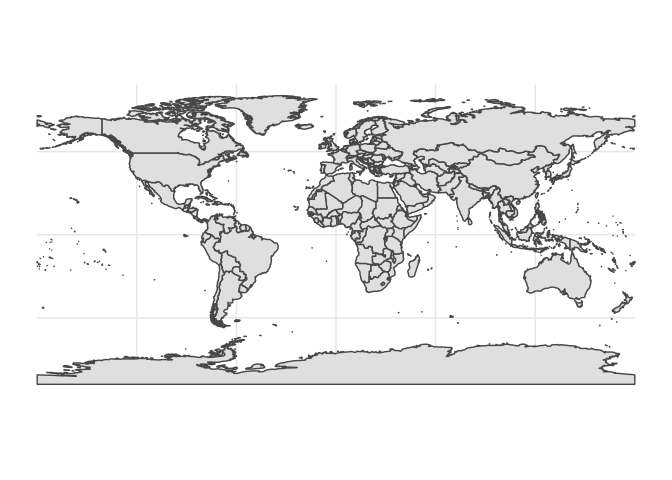
\includegraphics{GIS-workshop-for-participants-2020-0613JP_files/figure-latex/load-world-map-data-1.pdf}

Now, we want to plot Japan with some countries around it as our regional
map. We may want to indicate the countries by adding name label on it.
To do this, we need to get the center of the country for adding country
labels, and then specify which countries we want to show their names on
the map.

ここでは、日本を周辺のいくつかの国々とともに地域地図として描画し、国名を表示させたいと思います。そのために、中央に表示する国を指定し、表示範囲に含む国々を特定します。

\hypertarget{exercise-2-make-a-regional-map-7-minsux5b9fux7fd22ux5730ux57dfux5730ux56f3ux306eux4f5cux6210}{%
\subsection{Exercise 2: make a regional map (7
mins)/実習2:地域地図の作成}\label{exercise-2-make-a-regional-map-7-minsux5b9fux7fd22ux5730ux57dfux5730ux56f3ux306eux4f5cux6210}}

\begin{Shaded}
\begin{Highlighting}[]
\KeywordTok{library}\NormalTok{(tidyverse) }\CommentTok{#tidyverseのアクティベート}
\end{Highlighting}
\end{Shaded}

\begin{verbatim}
## -- Attaching packages ----------------------------------------------------------------------- tidyverse 1.3.0 --
\end{verbatim}

\begin{verbatim}
## v tibble  3.0.1     v dplyr   0.8.5
## v tidyr   1.0.2     v stringr 1.4.0
## v readr   1.3.1     v forcats 0.5.0
## v purrr   0.3.4
\end{verbatim}

\begin{verbatim}
## -- Conflicts -------------------------------------------------------------------------- tidyverse_conflicts() --
## x dplyr::filter() masks stats::filter()
## x dplyr::lag()    masks stats::lag()
\end{verbatim}

\begin{Shaded}
\begin{Highlighting}[]
\KeywordTok{library}\NormalTok{(sf) }\CommentTok{#sf(Simple Features)のアクティベート ※空間データを扱うため  }
\end{Highlighting}
\end{Shaded}

\begin{verbatim}
## Linking to GEOS 3.8.0, GDAL 3.0.4, PROJ 6.3.1
\end{verbatim}

\begin{Shaded}
\begin{Highlighting}[]
\NormalTok{country_centre_coords <-}
\StringTok{  }\KeywordTok{as_tibble}\NormalTok{(}\KeywordTok{st_coordinates}\NormalTok{(}\KeywordTok{st_centroid}\NormalTok{(world}\OperatorTok{$}\NormalTok{geometry))) }\CommentTok{# for the text labels/国名表示用}
\end{Highlighting}
\end{Shaded}

\begin{verbatim}
## Warning in st_centroid.sfc(world$geometry): st_centroid does not give correct
## centroids for longitude/latitude data
\end{verbatim}

\begin{Shaded}
\begin{Highlighting}[]
\NormalTok{world_points <-}
\StringTok{  }\NormalTok{world }\OperatorTok
\StringTok{  }\KeywordTok{bind_cols}\NormalTok{(country_centre_coords) }\OperatorTok
\StringTok{  }\KeywordTok{filter}\NormalTok{(name }\OperatorTok\StringTok{ }\KeywordTok{c}\NormalTok{(}\StringTok{"Japan"}\NormalTok{, }\StringTok{"China"}\NormalTok{, }\StringTok{"Korea"}\NormalTok{, }\StringTok{"Taiwan"}\NormalTok{, }\StringTok{"Russia"}\NormalTok{,}
                     \StringTok{"Philippines"}\NormalTok{, }\StringTok{"Vietnam"}\NormalTok{, }\StringTok{"Mongolia"}\NormalTok{)) }\CommentTok{# 表示に含める国々をworldオブジェクトから抽出}

\KeywordTok{library}\NormalTok{(shadowtext) }\CommentTok{#shadowtextのアクティベート ※ggplot2にshadowtextレイヤーを追加するため}

\CommentTok{# plot map/マップの描画}
\NormalTok{JP_NE_Asia <-}
\StringTok{  }\KeywordTok{ggplot}\NormalTok{(}\DataTypeTok{data =}\NormalTok{ world) }\OperatorTok{+}
\StringTok{  }\KeywordTok{geom_sf}\NormalTok{() }\OperatorTok{+}
\StringTok{  }\KeywordTok{geom_shadowtext}\NormalTok{(}\DataTypeTok{data=}\NormalTok{ world_points, }\CommentTok{# add texts/国名の追加  }
                  \KeywordTok{aes}\NormalTok{(}\DataTypeTok{x =}\NormalTok{ X, }\DataTypeTok{y =}\NormalTok{ Y,}
                      \DataTypeTok{label =}\NormalTok{ name),}
                  \DataTypeTok{color=}\StringTok{'black'}\NormalTok{,}
                  \DataTypeTok{bg.colour=}\StringTok{'white'}\NormalTok{,}
                  \DataTypeTok{size =} \DecValTok{3}\NormalTok{,}
                  \DataTypeTok{position =} \KeywordTok{position_nudge}\NormalTok{(}\DataTypeTok{y =} \DecValTok{0}\NormalTok{, }\DataTypeTok{x =} \DecValTok{3}\NormalTok{)) }\OperatorTok{+}
\StringTok{  }\KeywordTok{coord_sf}\NormalTok{(}\DataTypeTok{xlim =} \KeywordTok{c}\NormalTok{(}\DecValTok{95}\NormalTok{, }\DecValTok{175}\NormalTok{), }\CommentTok{# zoom in the area of interest/地図表示範囲の指定(x=経度,y=緯度)  }
           \DataTypeTok{ylim =} \KeywordTok{c}\NormalTok{(}\DecValTok{8}\NormalTok{, }\DecValTok{70}\NormalTok{), }
           \DataTypeTok{expand =} \OtherTok{FALSE}\NormalTok{) }\OperatorTok{+}\StringTok{ }\CommentTok{# match the limits we provide/指定範囲で切り抜き  }
\StringTok{  }\KeywordTok{scale_x_continuous}\NormalTok{(}\DataTypeTok{breaks =} \KeywordTok{seq}\NormalTok{(}\DecValTok{100}\NormalTok{, }\DecValTok{160}\NormalTok{, }\DataTypeTok{by =} \DecValTok{20}\NormalTok{)) }\OperatorTok{+}\StringTok{  }\CommentTok{#経緯線の間隔指定}
\StringTok{  }\KeywordTok{scale_y_continuous}\NormalTok{(}\DataTypeTok{breaks =} \KeywordTok{seq}\NormalTok{(}\DecValTok{20}\NormalTok{, }\DecValTok{65}\NormalTok{, }\DataTypeTok{by =} \DecValTok{20}\NormalTok{)) }\OperatorTok{+}
\StringTok{  }\KeywordTok{theme}\NormalTok{(}\DataTypeTok{axis.title.x =} \KeywordTok{element_blank}\NormalTok{(),}
        \DataTypeTok{axis.title.y =} \KeywordTok{element_blank}\NormalTok{())}

\NormalTok{JP_NE_Asia}
\end{Highlighting}
\end{Shaded}

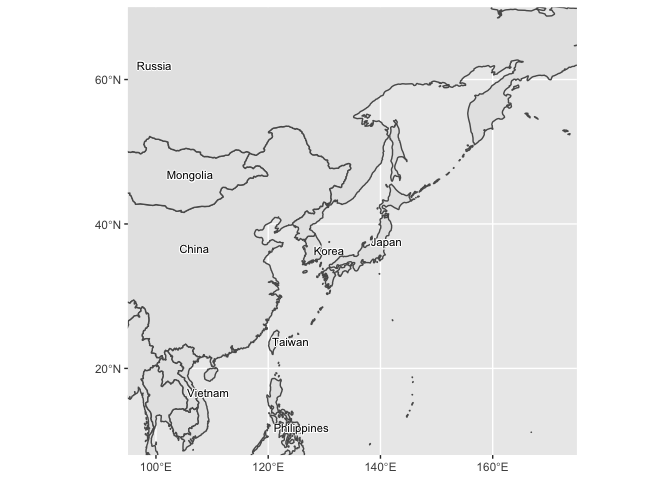
\includegraphics{GIS-workshop-for-participants-2020-0613JP_files/figure-latex/create-text-labels-1.pdf}

We also want to make a map with archaeological sites we are interested
in. Since we would add points for sites, we have to specify the
coordinates of site location first.

次に考古学遺跡の位置も追加したいと思います。そのためにはまず、遺跡の位置の座標を指定しなければなりません。

\hypertarget{exercise-3-make-site-map-7-mins}{%
\subsection{Exercise 3: make site map (7
mins)}\label{exercise-3-make-site-map-7-mins}}

\begin{Shaded}
\begin{Highlighting}[]
\CommentTok{# add site location/遺跡位置の追加  }
\NormalTok{site_location <-}
\StringTok{  }\KeywordTok{data.frame}\NormalTok{(}\DataTypeTok{location =} \KeywordTok{c}\NormalTok{(}\StringTok{"Daisen Kofun"}\NormalTok{, }\StringTok{"Todai-ji temple"}\NormalTok{),}
             \DataTypeTok{lon =} \KeywordTok{c}\NormalTok{(}\FloatTok{135.487953}\NormalTok{, }\FloatTok{135.839891}\NormalTok{),}
             \DataTypeTok{lat =} \KeywordTok{c}\NormalTok{(}\FloatTok{34.564503}\NormalTok{, }\FloatTok{34.688862}\NormalTok{))  }\CommentTok{#Daisen Kofun(大山古墳)とTodai-ji temple(東大寺)の位置情報をsite_locationに収納}

\KeywordTok{library}\NormalTok{(ggmap) }\CommentTok{#ggmapのアクティベート ※Rで地図表示を行なうため}
\end{Highlighting}
\end{Shaded}

\begin{verbatim}
## Google's Terms of Service: https://cloud.google.com/maps-platform/terms/.
\end{verbatim}

\begin{verbatim}
## Please cite ggmap if you use it! See citation("ggmap") for details.
\end{verbatim}

\begin{Shaded}
\begin{Highlighting}[]
\KeywordTok{library}\NormalTok{(ggspatial) }\CommentTok{#ggspatialのアクティベート ※ggplot2で地図・空間データを描画するため}
\KeywordTok{library}\NormalTok{(legendMap) }\CommentTok{#legendmapのアクティベート ※ggplot2で方位・スケールを描画するため}
\end{Highlighting}
\end{Shaded}

\begin{verbatim}
## Loading required package: maps
\end{verbatim}

\begin{verbatim}
## 
## Attaching package: 'maps'
\end{verbatim}

\begin{verbatim}
## The following object is masked from 'package:purrr':
## 
##     map
\end{verbatim}

\begin{verbatim}
## Loading required package: maptools
\end{verbatim}

\begin{verbatim}
## Loading required package: sp
\end{verbatim}

\begin{verbatim}
## Checking rgeos availability: TRUE
\end{verbatim}

\begin{verbatim}
## Loading required package: grid
\end{verbatim}

\begin{Shaded}
\begin{Highlighting}[]
\NormalTok{local_map <-}\StringTok{ }\KeywordTok{ggmap}\NormalTok{(}\KeywordTok{get_stamenmap}\NormalTok{(}\KeywordTok{rbind}\NormalTok{(}\KeywordTok{as.numeric}\NormalTok{(}\KeywordTok{c}\NormalTok{(}\FloatTok{135.3}\NormalTok{, }\FloatTok{34.3}\NormalTok{,}
                                                    \FloatTok{136.0}\NormalTok{, }\DecValTok{35}\NormalTok{))), }\DataTypeTok{zoom =} \DecValTok{10}\NormalTok{)) }\CommentTok{# define the range/地域地図の描画範囲(緯度経度で指定)とズームレベルを指定}
\end{Highlighting}
\end{Shaded}

\begin{verbatim}
## Source : http://tile.stamen.com/terrain/10/896/405.png
\end{verbatim}

\begin{verbatim}
## Source : http://tile.stamen.com/terrain/10/897/405.png
\end{verbatim}

\begin{verbatim}
## Source : http://tile.stamen.com/terrain/10/898/405.png
\end{verbatim}

\begin{verbatim}
## Source : http://tile.stamen.com/terrain/10/896/406.png
\end{verbatim}

\begin{verbatim}
## Source : http://tile.stamen.com/terrain/10/897/406.png
\end{verbatim}

\begin{verbatim}
## Source : http://tile.stamen.com/terrain/10/898/406.png
\end{verbatim}

\begin{verbatim}
## Source : http://tile.stamen.com/terrain/10/896/407.png
\end{verbatim}

\begin{verbatim}
## Source : http://tile.stamen.com/terrain/10/897/407.png
\end{verbatim}

\begin{verbatim}
## Source : http://tile.stamen.com/terrain/10/898/407.png
\end{verbatim}

\begin{verbatim}
## Source : http://tile.stamen.com/terrain/10/896/408.png
\end{verbatim}

\begin{verbatim}
## Source : http://tile.stamen.com/terrain/10/897/408.png
\end{verbatim}

\begin{verbatim}
## Source : http://tile.stamen.com/terrain/10/898/408.png
\end{verbatim}

\begin{Shaded}
\begin{Highlighting}[]
\NormalTok{site_Japan <-}\StringTok{ }
\StringTok{  }\NormalTok{local_map }\OperatorTok{+}
\StringTok{  }\KeywordTok{geom_point}\NormalTok{(}\DataTypeTok{data =}\NormalTok{ site_location, }\CommentTok{# add a layer of sites/遺跡のレイヤーを追加  }
             \KeywordTok{aes}\NormalTok{(}\DataTypeTok{x =}\NormalTok{ lon,}
                 \DataTypeTok{y =}\NormalTok{ lat),}
             \DataTypeTok{size =} \DecValTok{2}\NormalTok{,}
             \DataTypeTok{color =} \StringTok{"red"}\NormalTok{) }\OperatorTok{+}
\StringTok{  }\KeywordTok{geom_shadowtext}\NormalTok{(}\DataTypeTok{data =}\NormalTok{ site_location, }\CommentTok{# add texts }
                  \KeywordTok{aes}\NormalTok{(}\DataTypeTok{x =}\NormalTok{ lon,}
                      \DataTypeTok{y =}\NormalTok{ lat,}
                      \DataTypeTok{label =}\NormalTok{ location),}
                  \DataTypeTok{size =} \DecValTok{2}\NormalTok{,}
                  \DataTypeTok{position =} \KeywordTok{position_nudge}\NormalTok{(}\DataTypeTok{y =} \OperatorTok{-}\StringTok{ }\FloatTok{0.03}\NormalTok{),}
                  \DataTypeTok{check.overlap =} \OtherTok{TRUE}\NormalTok{) }\OperatorTok{+}
\StringTok{  }\KeywordTok{coord_sf}\NormalTok{(}\DataTypeTok{xlim =} \KeywordTok{c}\NormalTok{(}\FloatTok{135.3}\NormalTok{, }\DecValTok{136}\NormalTok{), }\CommentTok{# define the range/描画範囲を定義  }
           \DataTypeTok{ylim =} \KeywordTok{c}\NormalTok{(}\FloatTok{34.3}\NormalTok{, }\DecValTok{35}\NormalTok{),}
           \DataTypeTok{expand =} \OtherTok{FALSE}\NormalTok{) }\OperatorTok{+}
\StringTok{  }\KeywordTok{scale_x_continuous}\NormalTok{(}\DataTypeTok{breaks =} \KeywordTok{seq}\NormalTok{(}\FloatTok{135.3}\NormalTok{, }\DecValTok{136}\NormalTok{, }\DataTypeTok{by =} \FloatTok{0.2}\NormalTok{)) }\OperatorTok{+}\StringTok{ }
\StringTok{  }\KeywordTok{scale_y_continuous}\NormalTok{(}\DataTypeTok{breaks =} \KeywordTok{seq}\NormalTok{(}\FloatTok{24.3}\NormalTok{, }\DecValTok{35}\NormalTok{, }\DataTypeTok{by =} \FloatTok{0.2}\NormalTok{)) }\OperatorTok{+}\StringTok{  }\CommentTok{#経緯線の間隔を指定  }
\StringTok{  }\NormalTok{legendMap}\OperatorTok{::}\KeywordTok{scale_bar}\NormalTok{( }
    \DataTypeTok{lon =} \FloatTok{135.75}\NormalTok{,}
    \DataTypeTok{lat =} \FloatTok{34.32}\NormalTok{,}
    \DataTypeTok{legend_size =} \DecValTok{2}\NormalTok{,}
    \CommentTok{# distance of one section of scale bar, in km}
    \DataTypeTok{distance_lon =} \DecValTok{10}\NormalTok{,}
    \CommentTok{# height of the scale bar, in km}
    \DataTypeTok{distance_lat =} \DecValTok{1}\NormalTok{,}
    \CommentTok{# distance between scale bar and units, in km}
    \DataTypeTok{distance_legend =} \DecValTok{3}\NormalTok{,}
    \CommentTok{# units of scale bar}
    \DataTypeTok{dist_unit =} \StringTok{"km"}\NormalTok{,}
    \CommentTok{# add the north arrow}
    \DataTypeTok{orientation =} \OtherTok{TRUE}\NormalTok{,}
    \CommentTok{# length of N arrow, in km}
    \DataTypeTok{arrow_length =} \DecValTok{5}\NormalTok{,}
    \CommentTok{# distance between scale bar & base of N arrow, in km}
    \DataTypeTok{arrow_distance =} \DecValTok{3}\NormalTok{,}
    \CommentTok{# size of letter 'N' on N arrow, in km}
    \DataTypeTok{arrow_north_size =} \DecValTok{3}\NormalTok{) }\OperatorTok{+}
\StringTok{  }\KeywordTok{theme}\NormalTok{(}\DataTypeTok{axis.title.x =} \KeywordTok{element_blank}\NormalTok{(),}
        \DataTypeTok{axis.title.y =} \KeywordTok{element_blank}\NormalTok{())}
\end{Highlighting}
\end{Shaded}

\begin{verbatim}
## Coordinate system already present. Adding new coordinate system, which will replace the existing one.
\end{verbatim}

\begin{verbatim}
## Scale for 'x' is already present. Adding another scale for 'x', which will
## replace the existing scale.
\end{verbatim}

\begin{verbatim}
## Scale for 'y' is already present. Adding another scale for 'y', which will
## replace the existing scale.
\end{verbatim}

\begin{Shaded}
\begin{Highlighting}[]
\NormalTok{site_Japan}
\end{Highlighting}
\end{Shaded}

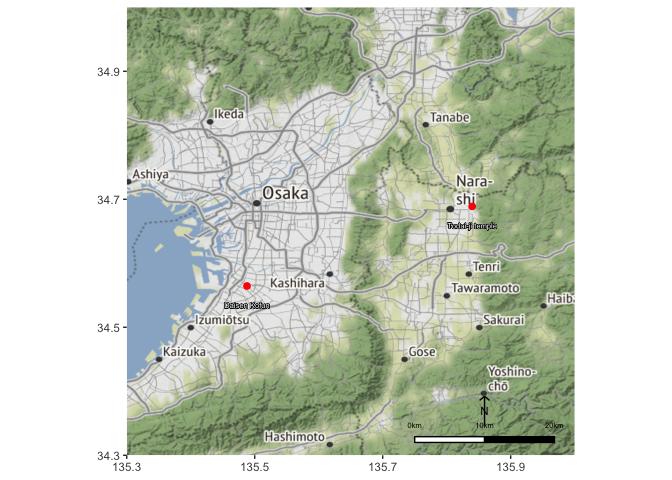
\includegraphics{GIS-workshop-for-participants-2020-0613JP_files/figure-latex/site-location-1.pdf}

(大阪と奈良を中心とした範囲の地図が描画され、大山古墳と東大寺の位置がプロットされます。もし2つの遺跡のドットとラベルが小さくて見えない場合は、165行目と171行目の\texttt{size=}の数値を大きくしてください。

We can save the map using ggsave function below the plot we would like
to save.

ggsave関数を利用して地図を保存することができます。

\begin{Shaded}
\begin{Highlighting}[]
\CommentTok{# save the map to your folder/フォルダに作成した地図を保存 }
\KeywordTok{ggsave}\NormalTok{(here}\OperatorTok{::}\KeywordTok{here}\NormalTok{(}\StringTok{"Japan-site-map.jpg"}\NormalTok{),}
       \DataTypeTok{width =} \DecValTok{60}\NormalTok{,}
       \DataTypeTok{height =} \DecValTok{60}\NormalTok{,}
       \DataTypeTok{dpi =} \DecValTok{300}\NormalTok{,}
       \DataTypeTok{units =} \StringTok{"mm"}\NormalTok{)}
\end{Highlighting}
\end{Shaded}

\hypertarget{spatial-data-manipulation-and-visualizationux7a7aux9593ux30c7ux30fcux30bfux306eux64cdux4f5cux3068ux53efux8996ux5316}{%
\section{Spatial data manipulation and
visualization/空間データの操作と可視化}\label{spatial-data-manipulation-and-visualizationux7a7aux9593ux30c7ux30fcux30bfux306eux64cdux4f5cux3068ux53efux8996ux5316}}

The raster data is DEM data downloaded from
\url{https://www.gsi.go.jp/kankyochiri/gm_japan_e.html}. We want to crop
the area that matches the site map from this DEM data. Here, we use
coordinates to create a data frame, convert it to a spatial object, and
then use it to crop the raster.

地図に使用したラスターデータは、国土地理院が提供するDEMデータです。遺跡地図で表示したい範囲のDEMデータを切り出したいと思います。位置座標でデータフレームを作成し、それを空間データオブジェクトに変換し、ラスターデータの切り抜きに使用します。

\hypertarget{exercise-4-crop-an-area-from-raster-data-7-minsux5b9fux7fd24ux30e9ux30b9ux30bfux30fcux30c7ux30fcux30bfux306eux5207ux308aux629cux304d}{%
\subsection{Exercise 4: crop an area from raster data (7
mins)/実習4:ラスターデータの切り抜き}\label{exercise-4-crop-an-area-from-raster-data-7-minsux5b9fux7fd24ux30e9ux30b9ux30bfux30fcux30c7ux30fcux30bfux306eux5207ux308aux629cux304d}}

\begin{Shaded}
\begin{Highlighting}[]
\KeywordTok{library}\NormalTok{(raster) }\CommentTok{#rasterのアクティベート ※ラスターデータ表示のため  }
\end{Highlighting}
\end{Shaded}

\begin{verbatim}
## 
## Attaching package: 'raster'
\end{verbatim}

\begin{verbatim}
## The following object is masked from 'package:dplyr':
## 
##     select
\end{verbatim}

\begin{verbatim}
## The following object is masked from 'package:tidyr':
## 
##     extract
\end{verbatim}

\begin{Shaded}
\begin{Highlighting}[]
\CommentTok{# read in data from data folder/フォルダからデータの読み込み}
\NormalTok{DEM_Japan <-}\StringTok{ }\KeywordTok{raster}\NormalTok{(}\StringTok{"data/workshop_data/jpn/el.tif"}\NormalTok{)  }\CommentTok{#ダウンロード済みデータをDEM_Japanに収納 ※日本全域  }

\CommentTok{# assign coordinate reference system/座標系の指定}
\KeywordTok{crs}\NormalTok{(DEM_Japan) <-}\StringTok{ "+proj=lcc +lat_1=41.03333333333333 +lat_2=40.66666666666666 +lat_0=40.16666666666666 +lon_0=-74 +x_0=300000 +y_0=0 +ellps=GRS80 +towgs84=0,0,0,0,0,0,0 +units=us-ft +no_defs"}
\end{Highlighting}
\end{Shaded}

\begin{verbatim}
## Warning in showSRID(uprojargs, format = "PROJ", multiline = "NO"): Discarded datum Unknown based on GRS80 ellipsoid in CRS definition,
##  but +towgs84= values preserved
\end{verbatim}

\begin{Shaded}
\begin{Highlighting}[]
\KeywordTok{plot}\NormalTok{(DEM_Japan) }\CommentTok{# take a look at raster data/ラスターデータの描画  }
\end{Highlighting}
\end{Shaded}

\begin{verbatim}
## Warning in showSRID(uprojargs, format = "PROJ", multiline = "NO"): Discarded datum Unknown based on GRS80 ellipsoid in CRS definition,
##  but +towgs84= values preserved

## Warning in showSRID(uprojargs, format = "PROJ", multiline = "NO"): Discarded datum Unknown based on GRS80 ellipsoid in CRS definition,
##  but +towgs84= values preserved
\end{verbatim}


\includegraphics{GIS-workshop-for-participants-2020-0613JP_files/figure-latex/get-raster-data-1.pdf}
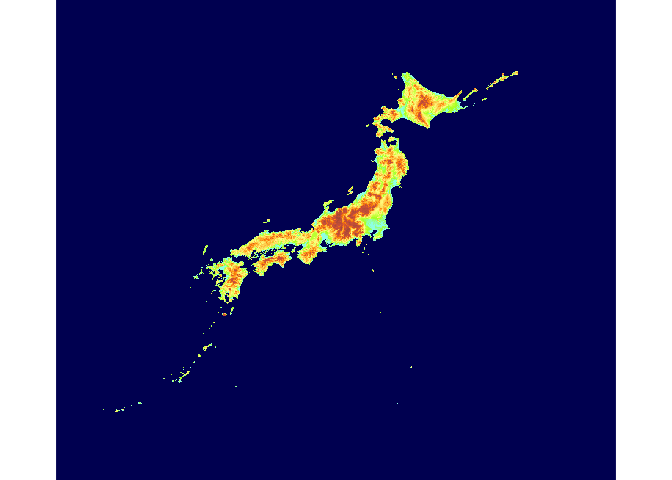
\includegraphics{GIS-workshop-for-participants-2020-0613JP_files/figure-latex/get-raster-data-2.pdf}

\begin{Shaded}
\begin{Highlighting}[]
\CommentTok{# define the area that we want to crop from the DEM/切り出したい範囲の定義  }
\NormalTok{x_coord <-}\StringTok{ }\KeywordTok{c}\NormalTok{(}\FloatTok{135.3}\NormalTok{, }\FloatTok{135.3}\NormalTok{, }\DecValTok{136}\NormalTok{, }\DecValTok{136}\NormalTok{, }\FloatTok{135.3}\NormalTok{)}
\NormalTok{y_coord <-}\StringTok{ }\KeywordTok{c}\NormalTok{(}\FloatTok{34.3}\NormalTok{, }\DecValTok{35}\NormalTok{, }\DecValTok{35}\NormalTok{, }\FloatTok{34.3}\NormalTok{, }\FloatTok{34.3}\NormalTok{)}
\NormalTok{xym <-}\StringTok{ }\KeywordTok{cbind}\NormalTok{(x_coord, y_coord)}

\KeywordTok{library}\NormalTok{(sp) }\CommentTok{#spのアクティベート ※空間データを取り扱うため  }
\NormalTok{p =}\StringTok{ }\KeywordTok{Polygon}\NormalTok{(xym) }\CommentTok{# convert the matrix to polygon/行列をポリゴンに変換  }
\NormalTok{ps =}\StringTok{ }\KeywordTok{Polygons}\NormalTok{(}\KeywordTok{list}\NormalTok{(p),}\DecValTok{1}\NormalTok{) }\CommentTok{# make lists/リストの作成  }
\NormalTok{sps =}\StringTok{ }\KeywordTok{SpatialPolygons}\NormalTok{(}\KeywordTok{list}\NormalTok{(ps)) }\CommentTok{# convert to Spatial Polygons/空間ポリゴンデータに変換  }
\KeywordTok{crs}\NormalTok{(sps) <-}\StringTok{ }\KeywordTok{crs}\NormalTok{(DEM_Japan) }\CommentTok{# define coordinate reference system/参照座標系の定義  }
\NormalTok{crop_DEM <-}\StringTok{ }\KeywordTok{crop}\NormalTok{(DEM_Japan, sps) }\CommentTok{# crop a raster to the extent of specified spatial object/設定した空間データオブジェクトによりラスターデータを切り出し  }
\end{Highlighting}
\end{Shaded}

\begin{verbatim}
## Warning in showSRID(uprojargs, format = "PROJ", multiline = "NO"): Discarded datum Unknown based on GRS80 ellipsoid in CRS definition,
##  but +towgs84= values preserved
\end{verbatim}

\begin{Shaded}
\begin{Highlighting}[]
\KeywordTok{plot}\NormalTok{(crop_DEM) }\CommentTok{#切り出したラスターデータの描画  }
\end{Highlighting}
\end{Shaded}

\begin{verbatim}
## Warning in showSRID(uprojargs, format = "PROJ", multiline = "NO"): Discarded datum Unknown based on GRS80 ellipsoid in CRS definition,
##  but +towgs84= values preserved
\end{verbatim}


\includegraphics{GIS-workshop-for-participants-2020-0613JP_files/figure-latex/get-raster-data-3.pdf}
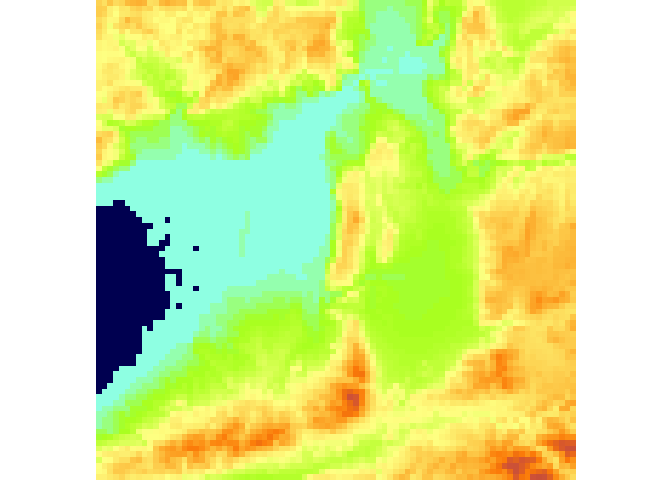
\includegraphics{GIS-workshop-for-participants-2020-0613JP_files/figure-latex/get-raster-data-4.pdf}

\begin{Shaded}
\begin{Highlighting}[]
\KeywordTok{summary}\NormalTok{(crop_DEM) }\CommentTok{#切り出したラスターデータの概要を表示  }
\end{Highlighting}
\end{Shaded}

\begin{verbatim}
##          el
## Min.      0
## 1st Qu.   4
## Median   14
## 3rd Qu.  33
## Max.    105
## NA's      0
\end{verbatim}

We can plot the raster data using ggplot function, which allows us to
modify axis, legend, and labels displayed on the plot. To use ggplot, we
need to convert the cropped raster to a dataframe.

ggplot関数を使用して、地図上に表示される軸や凡例、ラベルを編集し、ラスターデータを描画することができます。そのために、切り出したラスターデータをデータフレームに変換する必要があります。

\begin{Shaded}
\begin{Highlighting}[]
\CommentTok{# cover to a dataframe for ggplot/データフレームへの変換 ※ggplot用}
\NormalTok{crop_DEM_df <-}\StringTok{ }\KeywordTok{as.data.frame}\NormalTok{(crop_DEM, }\DataTypeTok{xy =} \OtherTok{TRUE}\NormalTok{)}
\CommentTok{# plot}
\KeywordTok{ggplot}\NormalTok{() }\OperatorTok{+}
\StringTok{  }\KeywordTok{geom_raster}\NormalTok{(}\DataTypeTok{data =}\NormalTok{ crop_DEM_df , }\KeywordTok{aes}\NormalTok{(}\DataTypeTok{x =}\NormalTok{ x, }\DataTypeTok{y =}\NormalTok{ y, }\DataTypeTok{fill =}\NormalTok{ el)) }\OperatorTok{+}
\StringTok{  }\KeywordTok{scale_fill_viridis_c}\NormalTok{(}\DataTypeTok{name =} \StringTok{"Elevation"}\NormalTok{) }\OperatorTok{+}
\StringTok{  }\KeywordTok{coord_quickmap}\NormalTok{() }\CommentTok{# plot faster/描画速度向上  }
\end{Highlighting}
\end{Shaded}

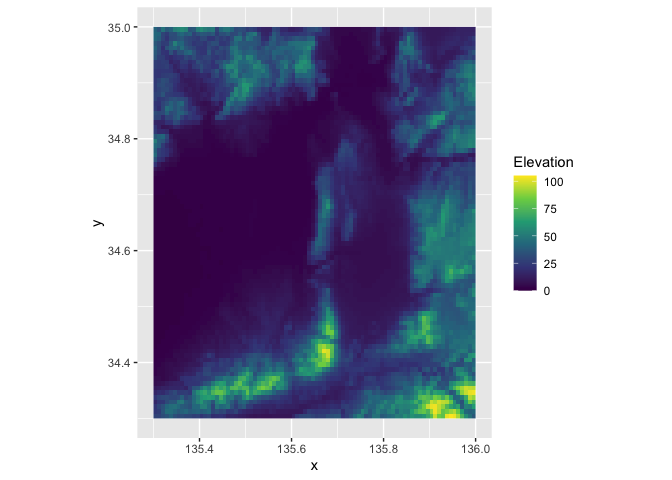
\includegraphics{GIS-workshop-for-participants-2020-0613JP_files/figure-latex/plot-raster-data-1.pdf}

Now, let's work on vector data and plot it on the raster. We import a
shapefile which contains site locations we want to explore (note: its
not a real data). We are curious about the distribution of
archaeological sites and how they relate to the elevation of this area.

続いて、ラスターデータの上にベクターデータを描画しましょう。検討したい遺跡の位置情報(ダミー:実在のデータではありません)を含むシェープファイルを読み込みます。この地域における標高と遺跡分布の関係に関心があります。

\hypertarget{exercise-5-explore-shapefile-and-map-it-on-the-raster-layer-7-minsux5b9fux7fd25ux30e9ux30b9ux30bfux30fcux30c7ux30fcux30bfux30ecux30a4ux30e4ux30fcux3067shapeux30d5ux30a1ux30a4ux30ebux3068ux5730ux56f3ux3092ux691cux8a0e}{%
\subsection{Exercise 5: explore shapefile and map it on the raster layer
(7
mins)/実習5:ラスターデータ・レイヤーでshapeファイルと地図を検討}\label{exercise-5-explore-shapefile-and-map-it-on-the-raster-layer-7-minsux5b9fux7fd25ux30e9ux30b9ux30bfux30fcux30c7ux30fcux30bfux30ecux30a4ux30e4ux30fcux3067shapeux30d5ux30a1ux30a4ux30ebux3068ux5730ux56f3ux3092ux691cux8a0e}}

\begin{Shaded}
\begin{Highlighting}[]
\NormalTok{crop_DEM_df <-}\StringTok{ }\KeywordTok{as.data.frame}\NormalTok{(crop_DEM, }\DataTypeTok{xy =} \OtherTok{TRUE}\NormalTok{)}
\CommentTok{# Example of archaeological sites/考古遺跡データのサンプル  }
\NormalTok{sites_location <-}\StringTok{ }\KeywordTok{st_read}\NormalTok{(}\StringTok{"data/workshop_data/sites_example.shp"}\NormalTok{) }\CommentTok{#shpファイル読込}
\end{Highlighting}
\end{Shaded}

\begin{verbatim}
## Reading layer `sites_example' from data source `C:\Users\Atsushi Noguchi\Documents\GitHub\Japan_GIS_workshop_202006_LW\data\workshop_data\sites_example.shp' using driver `ESRI Shapefile'
## Simple feature collection with 20 features and 2 fields
## geometry type:  POINT
## dimension:      XY
## bbox:           xmin: 135.412 ymin: 34.349 xmax: 135.951 ymax: 34.923
## CRS:            NA
\end{verbatim}

\begin{Shaded}
\begin{Highlighting}[]
\NormalTok{crop_DEM_df }\OperatorTok\StringTok{ }
\StringTok{  }\KeywordTok{ggplot}\NormalTok{() }\OperatorTok{+}\StringTok{ }
\StringTok{  }\KeywordTok{geom_raster}\NormalTok{(}\KeywordTok{aes}\NormalTok{(}\DataTypeTok{x =}\NormalTok{ x, }\DataTypeTok{y =}\NormalTok{ y, }\DataTypeTok{fill =}\NormalTok{ el)) }\OperatorTok{+}
\StringTok{  }\KeywordTok{geom_sf}\NormalTok{(}\DataTypeTok{data =}\NormalTok{ sites_location, }\KeywordTok{aes}\NormalTok{(}\DataTypeTok{color =}\NormalTok{ Period)) }\OperatorTok{+}\StringTok{ }\CommentTok{# add site shapefile/遺跡のシェープを追加  }
\StringTok{  }\KeywordTok{scale_color_manual}\NormalTok{(}\DataTypeTok{values=}\KeywordTok{c}\NormalTok{(}\StringTok{"red"}\NormalTok{, }\StringTok{"black"}\NormalTok{)) }\OperatorTok{+}\StringTok{ }\CommentTok{# change default color/基本色を変更  }
\StringTok{  }\KeywordTok{scale_fill_viridis_c}\NormalTok{(}\DataTypeTok{name =} \StringTok{"Elevation"}\NormalTok{) }\OperatorTok{+}
\StringTok{  }\KeywordTok{coord_sf}\NormalTok{() }\CommentTok{# all layers use a common CRS/共通のCRS(参照座標系)をすべてのレイヤーに使用  }
\end{Highlighting}
\end{Shaded}

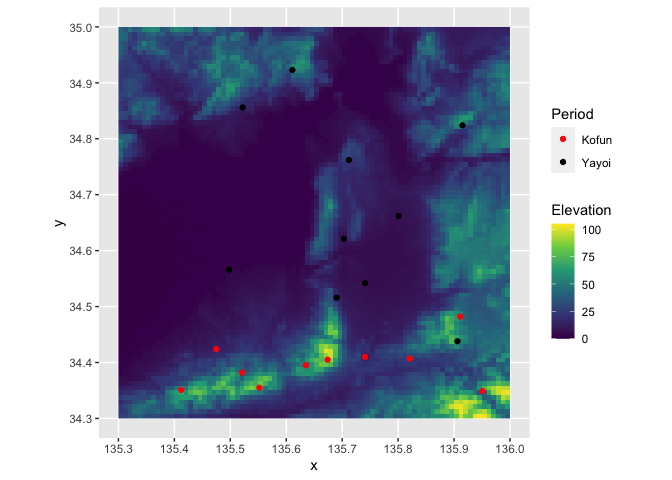
\includegraphics{GIS-workshop-for-participants-2020-0613JP_files/figure-latex/read-shapefile-1.pdf}

We are curious about the elevation of the locations of archaeological
sites, and would like to compare sites from two phases: Yayoi and Kofun.

弥生時代と古墳時代、2つの時期の遺跡の立地・標高を比較してみましょう。

\hypertarget{exercise-6-extract-elevation-and-make-a-plot-to-compare-sites-from-two-phases-5-minsux5404ux907aux8de1ux306eux6a19ux9ad8ux5024ux3092ux53d6ux5f97ux30572ux3064ux306eux6642ux4ee3ux3092ux6bd4ux8f03ux3059ux308bux30b0ux30e9ux30d5ux3092ux63cfux753b}{%
\subsection{Exercise 6: extract elevation and make a plot to compare
sites from two phases (5
mins)/各遺跡の標高値を取得し2つの時代を比較するグラフを描画}\label{exercise-6-extract-elevation-and-make-a-plot-to-compare-sites-from-two-phases-5-minsux5404ux907aux8de1ux306eux6a19ux9ad8ux5024ux3092ux53d6ux5f97ux30572ux3064ux306eux6642ux4ee3ux3092ux6bd4ux8f03ux3059ux308bux30b0ux30e9ux30d5ux3092ux63cfux753b}}

\begin{Shaded}
\begin{Highlighting}[]
\CommentTok{# convert sf (simple feature) to a spatial object/空間データ・オブジェクトをsf(simple feature)に変換  }
\NormalTok{sp_sites_location <-}\StringTok{ }\KeywordTok{as}\NormalTok{(sites_location, }\StringTok{"Spatial"}\NormalTok{)}

\CommentTok{# extract elevation for each site/各遺跡の標高を取得}
\NormalTok{elevation <-}\StringTok{ }\KeywordTok{extract}\NormalTok{(crop_DEM, sp_sites_location, }
                     \DataTypeTok{method =} \StringTok{"simple"}\NormalTok{) }\CommentTok{# use values for the cell a point falls in/遺跡が描画される位置のメッシュの情報をを使用  }
\NormalTok{sites_location <-}\StringTok{ }\KeywordTok{cbind}\NormalTok{(sites_location, elevation) }\CommentTok{#取得した標高値をデータ・オブジェクトに追加  }

\NormalTok{sites_location }\OperatorTok\StringTok{ }\CommentTok{#2つの時代の遺跡の標高の箱ひげ図を描画   }
\StringTok{  }\KeywordTok{ggplot}\NormalTok{(}\KeywordTok{aes}\NormalTok{(Period, elevation)) }\OperatorTok{+}\StringTok{ }
\StringTok{  }\KeywordTok{geom_boxplot}\NormalTok{() }\OperatorTok{+}
\StringTok{  }\KeywordTok{theme_minimal}\NormalTok{()}
\end{Highlighting}
\end{Shaded}

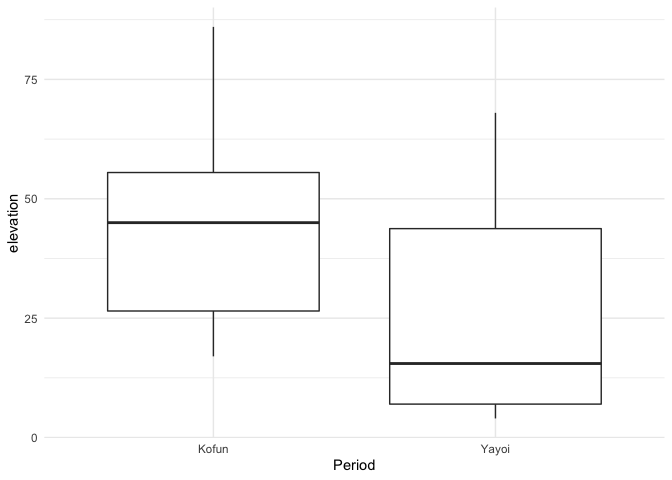
\includegraphics{GIS-workshop-for-participants-2020-0613JP_files/figure-latex/elevation-boxplot-two-phases-1.pdf}

\hypertarget{density-analysis-and-hypothesis-testingux5206ux5e03ux5bc6ux5ea6ux306eux5206ux6790ux3068ux4eeeux8aacux306eux691cux8a3c}{%
\section{Density analysis and hypothesis
testing/分布密度の分析と仮説の検証}\label{density-analysis-and-hypothesis-testingux5206ux5e03ux5bc6ux5ea6ux306eux5206ux6790ux3068ux4eeeux8aacux306eux691cux8a3c}}

We may want to know the distribution pattern of the sites across this
area. We can visualize the density to check any hot spots using kernal
density estimation.

次に、この地域の遺跡分布のパターンを検討したいと思います。カーネル密度推定により遺跡分布密度を可視化し「ホットスポット」があるかどうかを確認します。

\hypertarget{exercise-7-make-a-kernel-density-plot-7-minsux5b9fux7fd27ux30abux30fcux30cdux30ebux5bc6ux5ea6ux56f3ux306eux63cfux753b}{%
\subsection{Exercise 7: make a kernel density plot (7
mins)/実習7:カーネル密度図の描画}\label{exercise-7-make-a-kernel-density-plot-7-minsux5b9fux7fd27ux30abux30fcux30cdux30ebux5bc6ux5ea6ux56f3ux306eux63cfux753b}}

\begin{Shaded}
\begin{Highlighting}[]
\KeywordTok{library}\NormalTok{(spatstat)}
\end{Highlighting}
\end{Shaded}

\begin{verbatim}
## Loading required package: spatstat.data
\end{verbatim}

\begin{verbatim}
## Loading required package: nlme
\end{verbatim}

\begin{verbatim}
## 
## Attaching package: 'nlme'
\end{verbatim}

\begin{verbatim}
## The following object is masked from 'package:raster':
## 
##     getData
\end{verbatim}

\begin{verbatim}
## The following object is masked from 'package:dplyr':
## 
##     collapse
\end{verbatim}

\begin{verbatim}
## Loading required package: rpart
\end{verbatim}

\begin{verbatim}
## Registered S3 method overwritten by 'spatstat':
##   method     from
##   print.boxx cli
\end{verbatim}

\begin{verbatim}
## 
## spatstat 1.64-1       (nickname: 'Help you I can, yes!') 
## For an introduction to spatstat, type 'beginner'
\end{verbatim}

\begin{verbatim}
## 
## Attaching package: 'spatstat'
\end{verbatim}

\begin{verbatim}
## The following objects are masked from 'package:raster':
## 
##     area, rotate, shift
\end{verbatim}

\begin{Shaded}
\begin{Highlighting}[]
\KeywordTok{library}\NormalTok{(maptools)}
\NormalTok{crop_DEM_df <-}\StringTok{ }\KeywordTok{as.data.frame}\NormalTok{(crop_DEM, }\DataTypeTok{xy =} \OtherTok{TRUE}\NormalTok{)}

\CommentTok{# get two columns, one longitude and another is latitude/経度と緯度の取得  }
\NormalTok{sites_location_coords <-}
\StringTok{  }\NormalTok{sites_location }\OperatorTok\StringTok{ }
\StringTok{  }\KeywordTok{st_coordinates}\NormalTok{() }\OperatorTok\StringTok{ }
\StringTok{  }\NormalTok{as.data.frame }

\CommentTok{# convert to ppp object that represent a two-dimensional point pattern/2次元の点分布パターンを反映するpppオブジェクトを変換}
\NormalTok{sites_location_ppp <-}\StringTok{ }\KeywordTok{ppp}\NormalTok{(}\DataTypeTok{x =}\NormalTok{ sites_location_coords}\OperatorTok{$}\NormalTok{X,}
                          \DataTypeTok{y =}\NormalTok{ sites_location_coords}\OperatorTok{$}\NormalTok{Y,}
                          \KeywordTok{range}\NormalTok{(crop_DEM_df}\OperatorTok{$}\NormalTok{x), }\CommentTok{# set window, means the extent of an area}
                          \KeywordTok{range}\NormalTok{(crop_DEM_df}\OperatorTok{$}\NormalTok{y))}

\NormalTok{K1 <-}\StringTok{ }\KeywordTok{density}\NormalTok{(sites_location_ppp) }

\KeywordTok{plot}\NormalTok{(K1, }\DataTypeTok{main=}\OtherTok{NULL}\NormalTok{, }\DataTypeTok{las=}\DecValTok{1}\NormalTok{)}
\KeywordTok{contour}\NormalTok{(K1, }\DataTypeTok{add=}\OtherTok{TRUE}\NormalTok{)}
\end{Highlighting}
\end{Shaded}

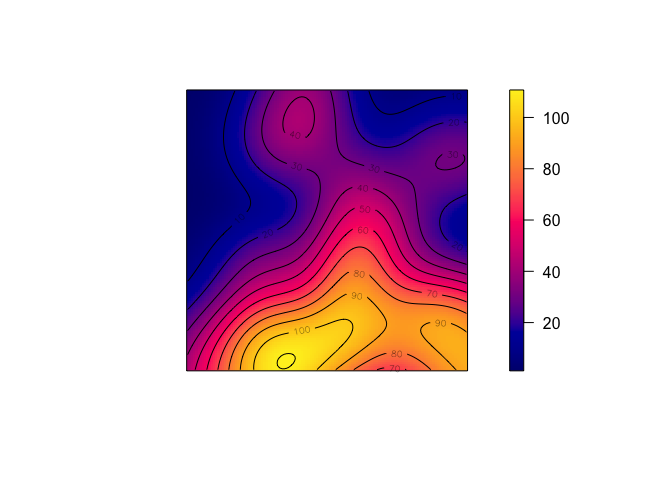
\includegraphics{GIS-workshop-for-participants-2020-0613JP_files/figure-latex/kernel-plot-all-sites-1.pdf}

Is the hot spots we observed significant? We can simulate the site
locations and testing our hypothesis to determine if the distribution is
random or not random.

明確な「ホットスポット」は確認できましたか?
次に遺跡位置をシミュレートし、分布パターンがランダムかどうかを検証します。

\hypertarget{exercise-8-simulation-and-plot-the-histogram-7-minsux5b9fux7fd28ux30b7ux30dfux30e5ux30ecux30fcux30b7ux30e7ux30f3ux3068ux30d2ux30b9ux30c8ux30b0ux30e9ux30e0ux306eux63cfux753b}{%
\subsection{Exercise 8: simulation and plot the histogram (7
mins)/実習8:シミュレーションとヒストグラムの描画}\label{exercise-8-simulation-and-plot-the-histogram-7-minsux5b9fux7fd28ux30b7ux30dfux30e5ux30ecux30fcux30b7ux30e7ux30f3ux3068ux30d2ux30b9ux30c8ux30b0ux30e9ux30e0ux306eux63cfux753b}}

\begin{Shaded}
\begin{Highlighting}[]
\CommentTok{# get the mean distance for our observation/観察結果から平均距離を取得}
\NormalTok{ann_p <-}\StringTok{ }\KeywordTok{mean}\NormalTok{(}\KeywordTok{nndist}\NormalTok{(sites_location_ppp, }\DataTypeTok{k=}\DecValTok{1}\NormalTok{))}
\NormalTok{n     <-}\StringTok{ }\DecValTok{1000} \CommentTok{# Number of simulations/シミュレーションの試行回数  }

\NormalTok{ann_r <-}\StringTok{ }\KeywordTok{vector}\NormalTok{(}\DataTypeTok{length =}\NormalTok{ n) }\CommentTok{# an object for storing simulated ANN values/シミュレーションしたANNをann_rに収納  }

\CommentTok{# simulation/シミュレーション}
\ControlFlowTok{for}\NormalTok{ (i }\ControlFlowTok{in} \DecValTok{1}\OperatorTok{:}\NormalTok{n)\{ }\CommentTok{#試行回数を指定(n=1000)}
\NormalTok{  rand_p   <-}\StringTok{ }\KeywordTok{rpoint}\NormalTok{(sites_location_ppp}\OperatorTok{$}\NormalTok{n, }
                     \DataTypeTok{win =} \KeywordTok{as.owin}\NormalTok{(crop_DEM_df))  }\CommentTok{# generate random point locations/ランダムな位置を生成}
\NormalTok{  ann_r[i] <-}\StringTok{ }\KeywordTok{mean}\NormalTok{(}\KeywordTok{nndist}\NormalTok{(rand_p, }\DataTypeTok{k=}\DecValTok{1}\NormalTok{))  }\CommentTok{# tally the ANN values/ANNを集計}
\NormalTok{\}}

\CommentTok{# plot the histogram and add our observed ANN value line/ヒストグラムを描画し、シミュレーション結果をのラインを追加}
\KeywordTok{hist}\NormalTok{(ann_r, }\DataTypeTok{main=}\OtherTok{NULL}\NormalTok{, }\DataTypeTok{las=}\DecValTok{1}\NormalTok{, }\DataTypeTok{breaks=}\DecValTok{40}\NormalTok{, }
     \DataTypeTok{col =} \StringTok{"bisque"}\NormalTok{, }
     \DataTypeTok{xlim =} \KeywordTok{range}\NormalTok{(ann_p, ann_r))}
\KeywordTok{abline}\NormalTok{(}\DataTypeTok{v =}\NormalTok{ ann_p, }\DataTypeTok{col=}\StringTok{"blue"}\NormalTok{) }\CommentTok{# the observed value}
\end{Highlighting}
\end{Shaded}

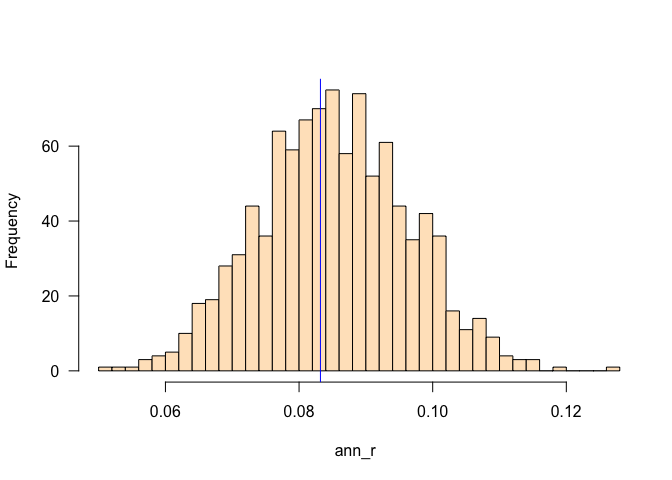
\includegraphics{GIS-workshop-for-participants-2020-0613JP_files/figure-latex/simulation-all-sites-1.pdf}

We have looked at the distribution of sites all together, but what if we
want to focus on sites from a phase; for example, we want to explore
Kofun period. We can filter out the phase we want and then use the same
method to test the Kofun sites.

ここでは全ての遺跡を検討しましたが、たとえば古墳時代の遺跡分布を検証するためには、遺跡分布データを時代でフィルターして同じ方法を適用します。

\hypertarget{quiz-do-the-kofun-sites-randomly-distributed-or-non-randomly-distributed-the-pattern-is-clustterd-or-dispersed-ux30afux30a4ux30baux53e4ux58b3ux6642ux4ee3ux907aux8de1ux306fux30e9ux30f3ux30c0ux30e0ux306aux5206ux5e03ux3067ux3059ux304b-ux5206ux5e03ux30d1ux30bfux30fcux30f3ux306fux30afux30e9ux30b9ux30bfux30fcux72b6ux3067ux3059ux304b-ux305dux308cux3068ux3082ux5206ux6563ux5206ux5e03ux3067ux3059ux304b}{%
\subsection{Quiz: Do the Kofun sites randomly distributed or
non-randomly distributed? The pattern is clustterd or dispersed?
/クイズ:古墳時代遺跡はランダムな分布ですか?
分布パターンはクラスター状ですか?
それとも分散分布ですか?}\label{quiz-do-the-kofun-sites-randomly-distributed-or-non-randomly-distributed-the-pattern-is-clustterd-or-dispersed-ux30afux30a4ux30baux53e4ux58b3ux6642ux4ee3ux907aux8de1ux306fux30e9ux30f3ux30c0ux30e0ux306aux5206ux5e03ux3067ux3059ux304b-ux5206ux5e03ux30d1ux30bfux30fcux30f3ux306fux30afux30e9ux30b9ux30bfux30fcux72b6ux3067ux3059ux304b-ux305dux308cux3068ux3082ux5206ux6563ux5206ux5e03ux3067ux3059ux304b}}

\begin{Shaded}
\begin{Highlighting}[]
\NormalTok{sites_location_coords_kofun <-}\StringTok{ }\CommentTok{#古墳時代遺跡のカーネル密度推定と描画  }
\StringTok{  }\NormalTok{sites_location }\OperatorTok\StringTok{ }
\StringTok{  }\KeywordTok{st_coordinates}\NormalTok{() }\OperatorTok\StringTok{ }
\StringTok{  }\KeywordTok{as.data.frame}\NormalTok{ () }\OperatorTok\StringTok{ }
\StringTok{  }\KeywordTok{bind_cols}\NormalTok{(sites_location) }\OperatorTok\StringTok{ }
\StringTok{  }\KeywordTok{filter}\NormalTok{(Period }\OperatorTok{==}\StringTok{ "Kofun"}\NormalTok{)}

\NormalTok{sites_location_ppp_kofun <-}\StringTok{ }\NormalTok{(}\KeywordTok{ppp}\NormalTok{(}\DataTypeTok{x =}\NormalTok{ sites_location_coords_kofun}\OperatorTok{$}\NormalTok{X,}
                                 \DataTypeTok{y =}\NormalTok{ sites_location_coords_kofun}\OperatorTok{$}\NormalTok{Y,}
                                 \KeywordTok{range}\NormalTok{(crop_DEM_df}\OperatorTok{$}\NormalTok{x),}
                                 \KeywordTok{range}\NormalTok{(crop_DEM_df}\OperatorTok{$}\NormalTok{y))) }

\NormalTok{K2 <-}\StringTok{ }\KeywordTok{density}\NormalTok{(sites_location_ppp_kofun) }

\KeywordTok{plot}\NormalTok{(K2, }\DataTypeTok{main=}\OtherTok{NULL}\NormalTok{, }\DataTypeTok{las=}\DecValTok{1}\NormalTok{)}
\KeywordTok{contour}\NormalTok{(K2, }\DataTypeTok{add=}\OtherTok{TRUE}\NormalTok{)}
\end{Highlighting}
\end{Shaded}

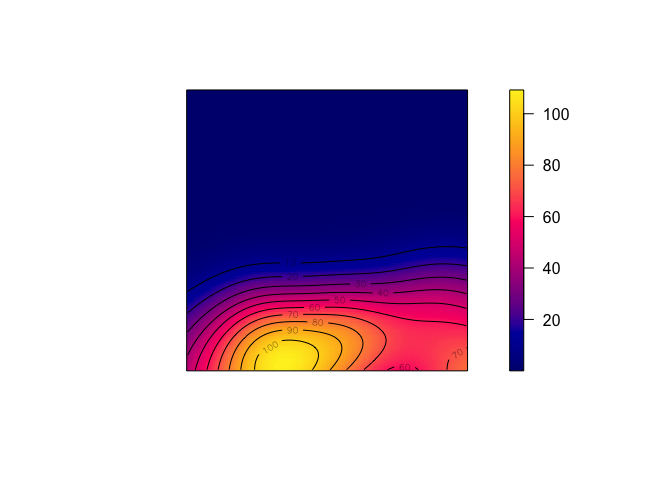
\includegraphics{GIS-workshop-for-participants-2020-0613JP_files/figure-latex/kernel-plot-kofun-1.pdf}

\begin{Shaded}
\begin{Highlighting}[]
\NormalTok{ann_p <-}\StringTok{ }\KeywordTok{mean}\NormalTok{(}\KeywordTok{nndist}\NormalTok{(sites_location_ppp_kofun, }\DataTypeTok{k=}\DecValTok{1}\NormalTok{))}
\NormalTok{n     <-}\StringTok{ }\DecValTok{1000} \CommentTok{# Number of simulations}

\NormalTok{ann_r <-}\StringTok{ }\KeywordTok{vector}\NormalTok{(}\DataTypeTok{length =}\NormalTok{ n) }\CommentTok{# an object for storing simulated ANN values}

\CommentTok{# simulation}
\ControlFlowTok{for}\NormalTok{ (i }\ControlFlowTok{in} \DecValTok{1}\OperatorTok{:}\NormalTok{n)\{}
\NormalTok{  rand_p   <-}\StringTok{ }\KeywordTok{rpoint}\NormalTok{(sites_location_ppp_kofun}\OperatorTok{$}\NormalTok{n, }
                     \DataTypeTok{win =} \KeywordTok{as.owin}\NormalTok{(crop_DEM_df))  }\CommentTok{# Generate random point locations}
\NormalTok{  ann_r[i] <-}\StringTok{ }\KeywordTok{mean}\NormalTok{(}\KeywordTok{nndist}\NormalTok{(rand_p, }\DataTypeTok{k=}\DecValTok{1}\NormalTok{))  }\CommentTok{# Tally the ANN values}
\NormalTok{\}}

\CommentTok{# plot the histogram and add our observed ANN value line}
\KeywordTok{hist}\NormalTok{(ann_r, }\DataTypeTok{main=}\OtherTok{NULL}\NormalTok{, }\DataTypeTok{las=}\DecValTok{1}\NormalTok{, }\DataTypeTok{breaks=}\DecValTok{40}\NormalTok{, }
     \DataTypeTok{col =} \StringTok{"bisque"}\NormalTok{, }
     \DataTypeTok{xlim =} \KeywordTok{range}\NormalTok{(ann_p, ann_r))}
\KeywordTok{abline}\NormalTok{(}\DataTypeTok{v =}\NormalTok{ ann_p, }\DataTypeTok{col=}\StringTok{"blue"}\NormalTok{)}
\end{Highlighting}
\end{Shaded}

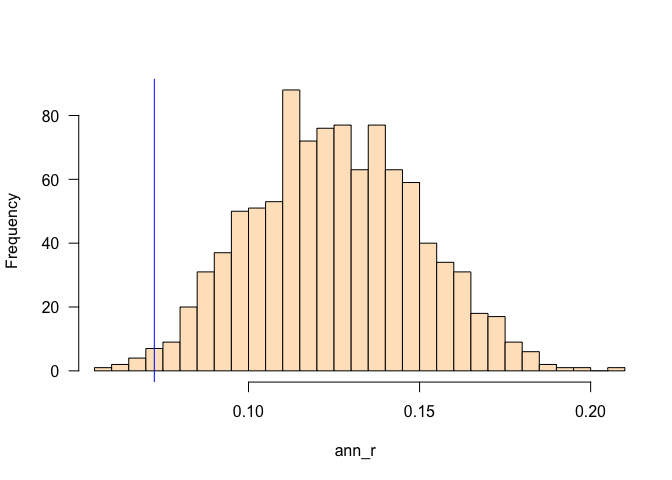
\includegraphics{GIS-workshop-for-participants-2020-0613JP_files/figure-latex/simulation-kofun-1.pdf}

\end{document}
